\documentclass[11pt]{article}
\usepackage[utf8]{inputenc}

\title{Recipe Recommendations}
\author{Easton Potokar}
\date{March 2020}

\usepackage{graphicx}
\usepackage{natbib}
\usepackage{amsmath}
\usepackage{xcolor}
\usepackage[margin=1.5in]{geometry}
\usepackage[colorlinks = true,
            linkcolor = blue,
            urlcolor  = blue,
            citecolor = blue,
            anchorcolor = blue]{hyperref}
            
\newcommand\todo[1]{\textcolor{red}{TODO: #1 \\}}
% \renewcommand\todo[1]{}

\newcommand*\textfrac[2]{
  \frac{\text{#1}}{\text{#2}}
}

\begin{document}

\maketitle

\begin{abstract}
    We seek to explore making a personalized recipe recommendation system based on ingredients, tags, and past user reviews. We analyze both the accuracy of the recommendations as well as the temporal complexity of making them. We find that we can make very accurate recommendations to satisfy what cravings people may have and those they didn't know they had.
\end{abstract}

\section{Problem Statement and Motivation}
Machine Learning algorithms that make recommendations to users are becoming more and more common and are seen all over the internet for movies, friends, web searches, etc. A less common application is for recipe suggestions. Is it possible to find a perfect recipe for someone given their past preferences of foods? Can we do it in fast enough so we don't lose their interest?

This has been attempted using matrix factorization \cite{mf}, which essentially utilizes both components of an
SVD decomposition. There has also been work done to use a hybrid approach that utilizes both the reviews of users and the attributes of the recipes, whereas more traditional methods use one or the other \cite{india}.  We seek to continue along this path of more traditional methods, while also analyzing the speed of our algorithms to see how viable they would be in production.


\section{Data}
\begin{figure}[t]
\centering
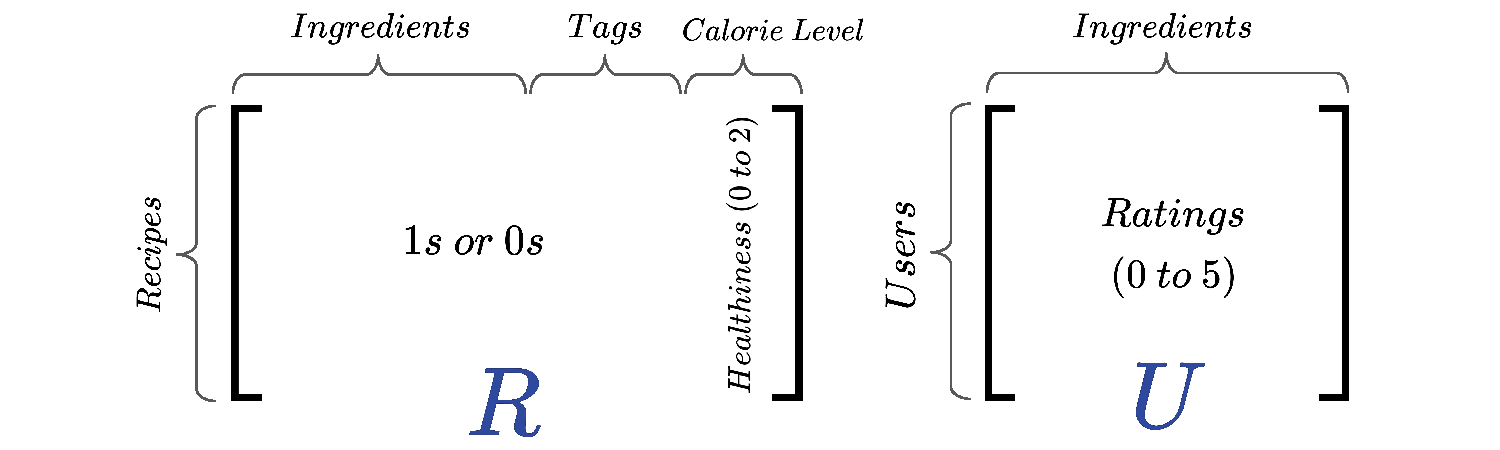
\includegraphics[width=0.9\textwidth]{figs/data.pdf}
\caption{Data Overview}
\label{fig:data_overview}
\end{figure}

Our data was gathered from \cite{data}, whose dataset can be found \href{https://www.kaggle.com/shuyangli94/food-com-recipes-and-user-interactions}{here}. The data consists of more than 180 thousand recipes (made up of their ingredients, calorie level, and various tags describing them), and 700 thousand user reviews of the 180 thousand recipes all scraped from Food.com  and ranging from 1 to 5 stars. The original authors of the data used various natural language processing techniques to parse the recipes into about 8 thousand unique ingredients, around 500 unique tags, and a calorie level that is a 0, 1, or 2 denoting low-calorie to high-calorie recipes. To visualize what we're saying, see Figure \ref{fig:data_overview}. We denote the recipe dataset as $R$ and the user dataset as $U$ throughout the rest of the paper.

The data appears to be very reliable, having been scraped directly from Food.com with the scraper being publicly available on github \cite{data_scraper}. Furthermore, it was used in a published research article, so one would hope everything was done ethically and correctly. The dataset is plenty large enough to give use meaningful answers to our questions and should be able to make a fairly robust recommendation system.


\section{Ethical Ramifications}
As with all recommendation systems, we must be careful of what sort of bias we program into our algorithms. It would be very easy to heavily weight the algorithms to favor low-calorie recipes (healthier options) in an effort to push the public towards eating more healthy. While this would likely be well intentioned, in a way it is removing one's freedom of options, and is manipulating users' behavior. Many similar biases must also be carefully considered, whether it be toward a certain ingredient/brand (company sponsorship), a certain ethnic preference (potentially racist), etc.

\section{Methods}

\subsection{Data Preparation}
\begin{figure}[t]
\centering
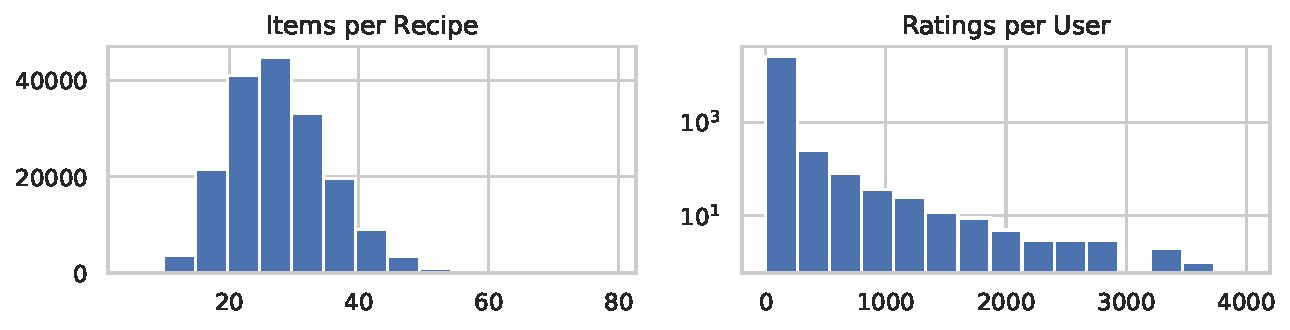
\includegraphics[width=0.9\textwidth]{figs/dist.pdf}
\caption{Data Statistics}
\label{fig:dist}
\end{figure}

Our data is on the format as seen in Figure \ref{fig:data_overview}. This is a far from perfect solution. Note that the importance of a recipe having salt will be just as important as a recipe having jasmine or a jalapeno pepper. Commonly used in document classification, we use "TF-IDF" to help with this problem. In our case, we change each entry using the conversion (where item means either ingredient/tag):

$$\textfrac{Quantity of $i$th item}{Total \# of items in Recipe} * \log \Big( \textfrac{Total \# of Recipes}{\# of Recipes with $i$th item} \Big)$$

We perform the same transformation on the user dataset, replacing item with rating, and recipes with users. Throughout this document we analyze our data in both forms in order to visualize which data format helps the algorithms perform the best. We denoted these datasets as $Rhat$ and $Uhat$ as compared to $R$ and $U$ for the original datasets.

To give ourselves a little intuition, we also visualize the distributions of how many items a recipe has and how many recipes a user has rated. This can be seen in Figure \ref{fig:dist}.


\subsection{Recommendation Process}
Most recommendation systems or "filtering" systems are considered either content-based or collaborative-based filtering. Content-based systems make recommendations on attributes of the items; in our case, this would be ingredients and tags of our recipes. Collaborative-based filtering uses the history of other users who are similar to us to recommend items. We'll explore using both. Our workflows will be as shown in Figure \ref{fig:flow}.

\begin{figure}[t]
\centering
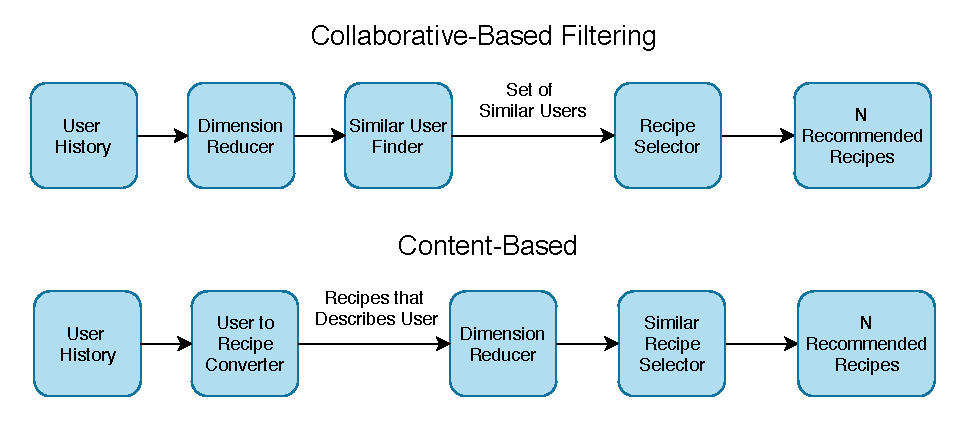
\includegraphics[width=1\textwidth]{figs/flow.pdf}
\caption{Recommendation Systems Flow}
\label{fig:flow}
\end{figure}

\subsubsection{Collaborative-Based Filtering}

It's here that we'll use our new algorithm, DBSCAN, which stands for density-based spatial clustering of applications with noise. It clusters by defining core samples, which are data points that have a minimum number of samples within a certain epsilon. It then recursively tests the samples within that epsilon to see if they're core samples as well, and continues iterating until finished. This allows DBSCAN to detect non-convex clusters unlike KMeans and GMM, but still be relatively faster that MinCut and t-SNE.

We'll go over what was attempted in each step of collaborative-based filtering
\begin{enumerate}
    \item \textbf{Dimension Reducer}. PCA, LDA, NMF and Kernelized PCA were all used. Probablistic PCA and Sparse PCA were also attempted, but don't play well with sparse input. Kernelized PCA was also too computationally expensive and often abandoned.
    \item \textbf{User Finder}. We tried various algorithms for this:
    \begin{itemize}
        \item k Nearest Neighbor (kNN).
        \item Various Clustering Algorithms. Return all other users found in same cluster. Attempted using KMeans, GMM, MinCut, and DBSCAN.
        \item Combination of clustering and kNN. Return k nearest neighbors found in cluster. Could potentially be more computationally effective.
    \end{itemize}
    We also take care to make sure our user finder doesn't return the input user.
    \item \textbf{Recipe Selector}. Taking the users passed to it, count number of times recipes are rated by user set along with their rating. Choose from among recipes by:
    \begin{itemize}
        \item Sorting by sum of ratings and return largest N sums
        \item Sorting by frequency and then by average rating. Return N largest.
        \item Sorting by average rating and then frequency. Return N largest.
    \end{itemize}
\end{enumerate}

Note if our algorithm returns too few recommendations, (ie a cluster ends up being a singleton or something of the sort), we simply fill in the rest with random recipes. 

\subsubsection{Content-Based Filtering}
We'll go over what was attempted in each step of content-based filtering
\begin{enumerate}
    \item \textbf{User to Recipe Converter}. We attempt this in two ways:
    \begin{itemize}
        \item Take all recipes with rating from user above a threshold. This method keeps each recipe separate (SR).
        \item Take all ingredients from recipes with rating from user above a threshold and combine into one huge recipe. (TR) 
    \end{itemize}
    \item \textbf{Dimension Reducer}. Dimensions were reduced in the same way as in the Collaborative-Based Approach.
    \item \textbf{Similar Recipe Selector}. In the case where the set of user describing recipes is a singleton, simply take the N NNs. In the case it isn't, take k NNs of each recipe and return the N most frequent.
\end{enumerate}

\subsubsection{Scoring}

To evaluate our models, we removed around 100 thousand reviews from random users. We will then take in the user as input and try to recommend the removed recipe that we know they rated or a recipe similar to it.

To quantitatively define how good a prediction is, we use two different loss functions.  Let $R$ be the recommended recipe, $G$ the goal recipe and $I_R$, $I_G$ be the set of items that each has. We define our loss functions as:
\begin{align}
    Int(R,G) = |I_R \cap I_G| && Com(R,G) = -|(I_R \cap I_G)^C|
\end{align}
We desire to maximize both. $Int(R,G)$ rewards us for correctly recommending items; $Com(R,G)$ punishes us for recommending incorrect items. Sometimes we may recommend something with cheddar cheese instead of American cheese and $Com(R,G)$ punishes that, even though it's likely close enough. Similarly, $Int(R,G)$ rewards recipes that have many ingredients. Using both gives us more insight on how our algorithms perform.

To get our total loss, we simply take the mean of all N (we have arbitrarily chosen N=5 for our tests) recommendations and then the mean of all the data points together.


\section{Results}

We ran a grid search over each combination of dimension reducer and similarity finder to find the best hyperparameters for each combination of the two. We also timed both the fitting as well as the prediction steps to be able to see which methods are actually feasible in practice. We did this separately for both the intersection and the complement metric to see how each could be maximized. The results can be seen in Figures \ref{fig:user_results}, \ref{fig:recipe_results} and \ref{fig:best}.

After a few test were done, we found that the best recipe selector for collarborative-based filtering was sorting by sum of ratings, almost uniformly. To help narrow down our search, we used it exclusively. 

Certain combinations had to be abandoned as well due to high processing requirements that just didn't make them feasible in practice. This includes kernelized PCA with content-based filtering, as well as using MinCut along with NN. 

As a baseline, we tested the performance of randomly predicting N recipes and recommending the N most popular recipes. Random recipes got 7.66 and -39.12 and popular recipes got 9.58 and -42.515, in the intersection and complement metrics respectively.


We also include the best results in each category in Figure \ref{fig:best}. We calculated best overall by averaging their rank in each metric.

\section{Analysis}

\subsection{Collaborative-Based Approach}

\begin{figure}[b!]
\centering
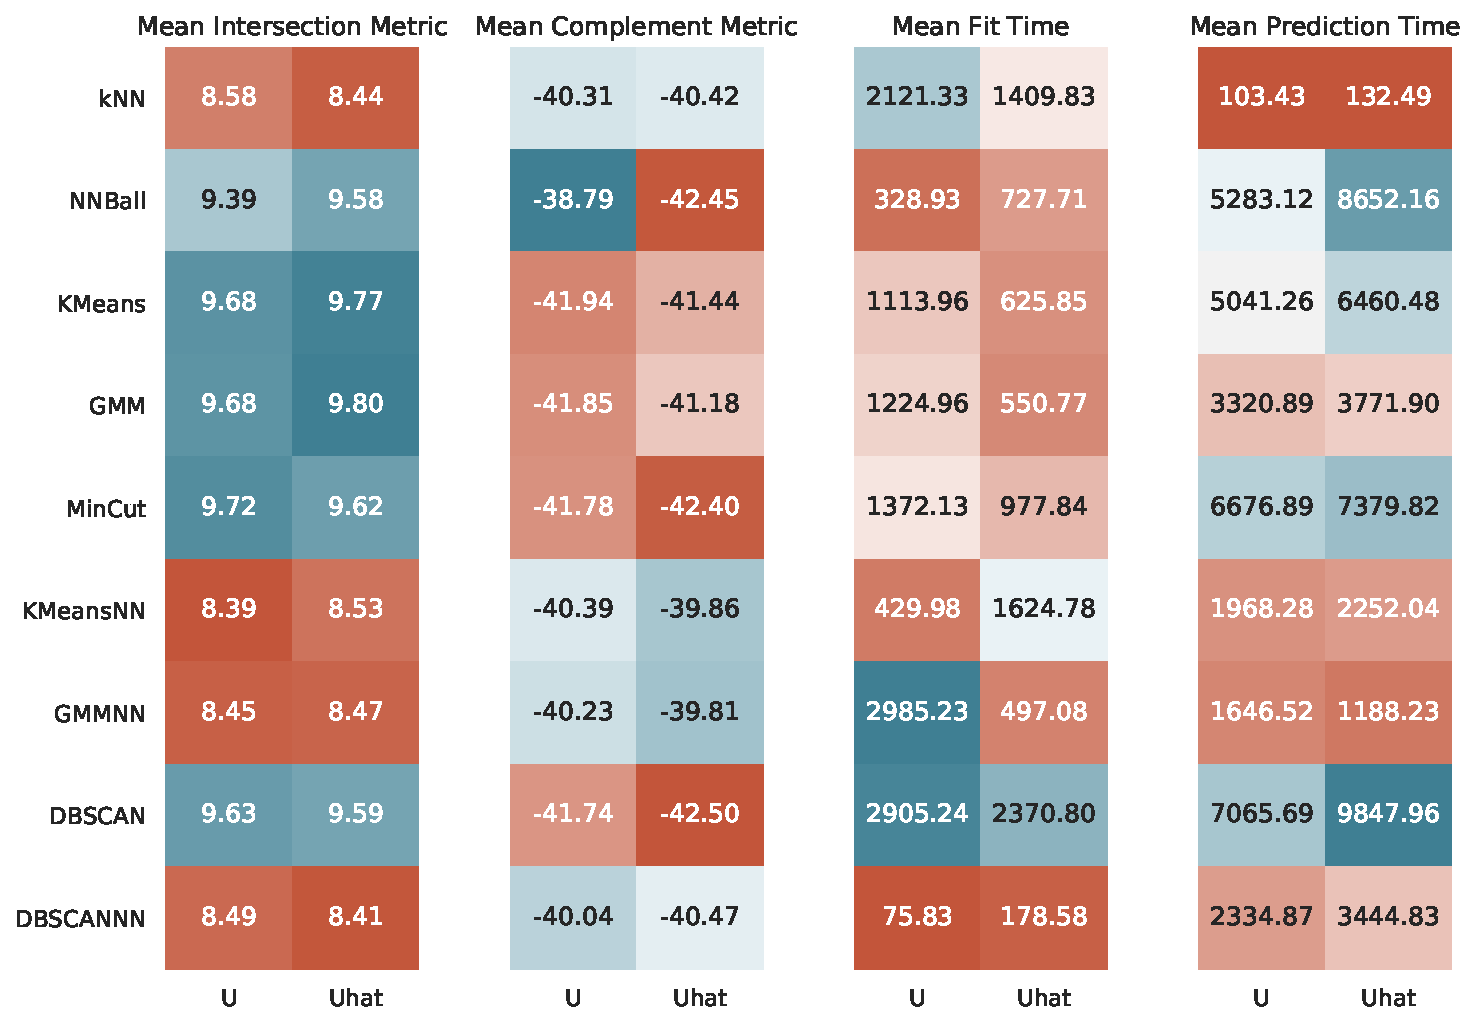
\includegraphics[width=1\textwidth]{figs/user_rdr.pdf}
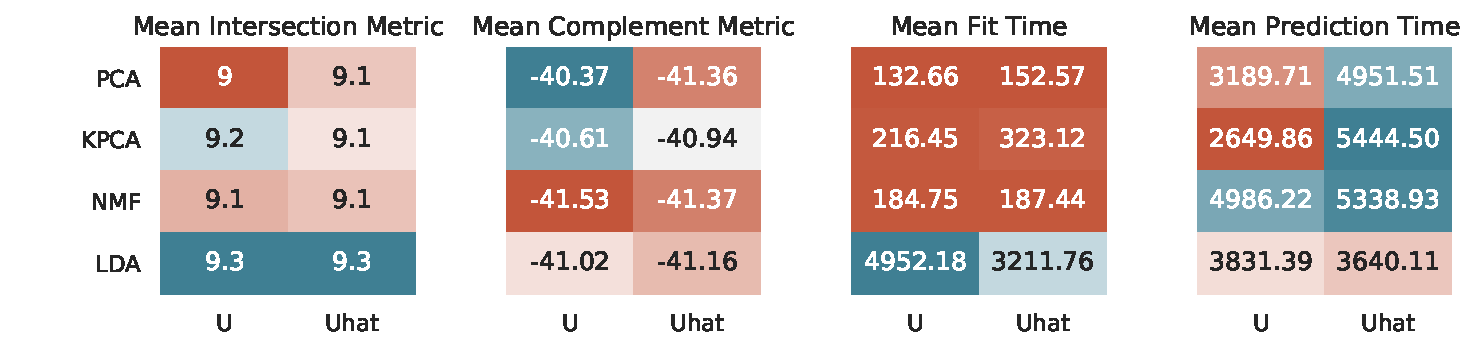
\includegraphics[width=1\textwidth]{figs/user_dr.pdf}
\caption{Comparison of Collaboration-Based Recommendation Algorithms}
\label{fig:user_results}
\end{figure}

First note that nearly none of these algorithms were particularly good in the complement metric. This means that on average, no particular algorithm was extremely adept at the complement metric under all circumstances, but doesn't mean that a certain combination won't perform extremely well.

Also, the clustering algorithms all did almost uniformly well, with very little separating them. This surprises me since I expected the clusters to be relatively non-convex, but based on these results, I would actually assume that most of the resulting clusters are convex. They performed a little better than recommending popular recipes, and I expect would bring better variety to users as well, making them particularly worth having around. It also appears the shortcomings of kNN also fell upon the combo cluster and kNN algorithms as they performed better than random, but still worse than just recommending popular algorithms. I would also guess that NNBall essentially acted as a "local" cluster by just selecting everything within a radius of itself, thereby circumventing the shortcomings of kNN (which may reach very far away to select a neighbor).

Also, the choice of data, original or TF-IDF, made very minimal difference in the results, which is extremely surprising. This could be due to most users having rated so few recipes out of the total amount of recipes, that it ends up looking like they're close/not close regardless of the data. 

Also note that the choice of dimension reducer had little to no effect on average either. Again, this doesn't mean a certain combination of dimension reducer and similar user selector might be dynamite, but as a whole, it didn't matter too much.

\subsection{Content-Based Approach}

\begin{figure}[b!]
\centering
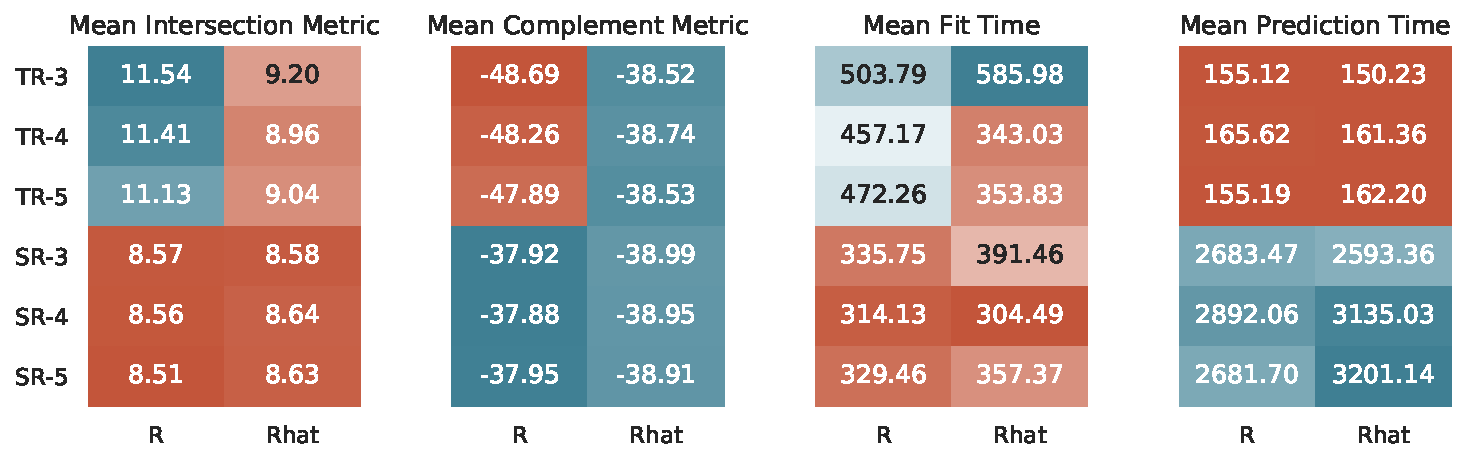
\includegraphics[width=1\textwidth]{figs/recipe_rdr.pdf}
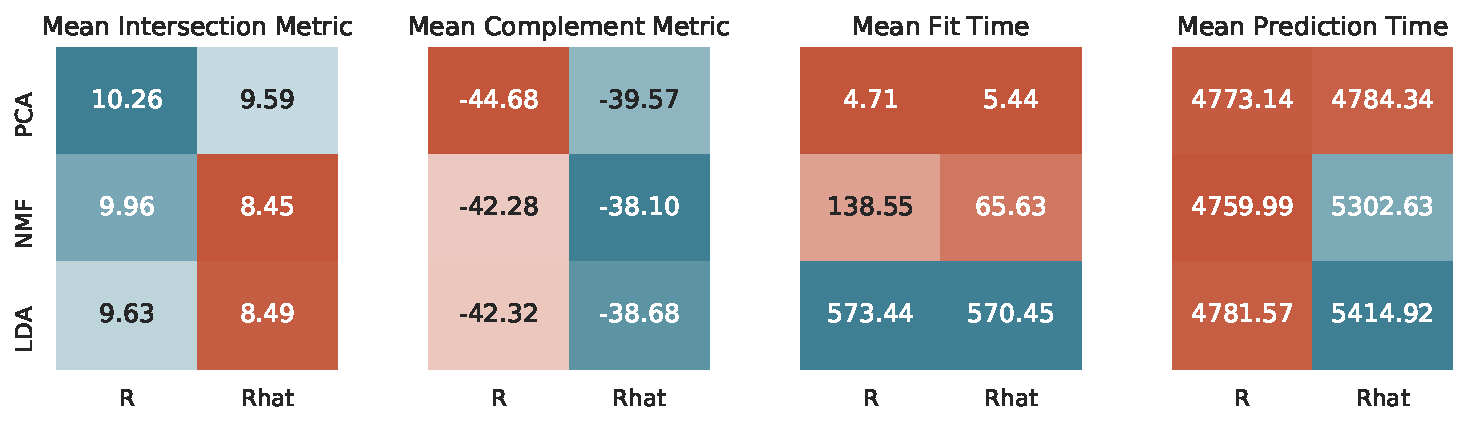
\includegraphics[width=1\textwidth]{figs/recipe_dr.pdf}
\caption{Comparison of Content-Based Recommendation Algorithms}
\label{fig:recipe_results}
\end{figure}

Right off the bat, it can be seen that the mashing all previously liked ingredients of a user into a recipe and finding similar ones (TR) likely just sought out recipes that have many many ingredients, which means it should probably be avoided. On the other hand, separating out the recipes had the opposite effect, performing extremely well in the complement metric and poorly in the intersection metric.

Once again, the choice of dimension reducers appears to mostly be a wash.

Finally, the choice of data in this scenario did play a huge role in the results. Notice that the use of TF-IDF really improved performance in the complement metric, possibly playing a pretty active role in transforming the vector space.  
\begin{figure}[b!]
\centering
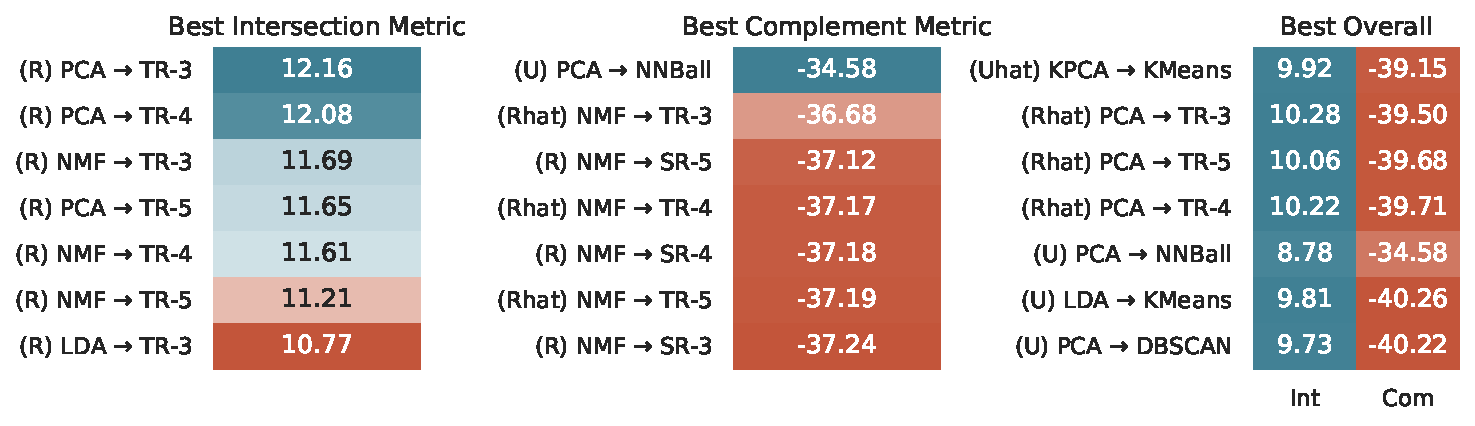
\includegraphics[width=1\textwidth]{figs/best_metric.pdf}
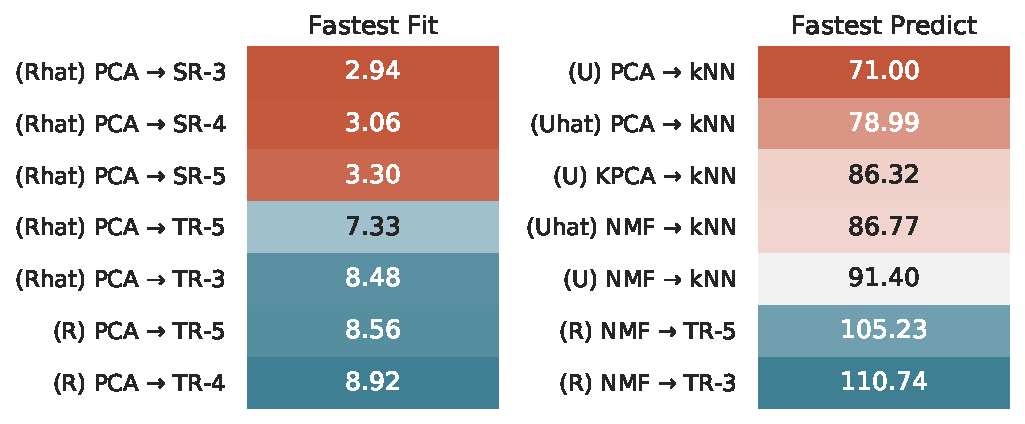
\includegraphics[width=0.63\textwidth]{figs/best_time.pdf}
\caption{Best Results}
\label{fig:best}
\end{figure}

\section{Conclusion}

Recommendations systems are common all over the web from Netflix to eBay. One space where the usefulness of these hasn't been researched extensively is the food recipe industry. In our analysis, we found no clear cut perfect algorithm in all scenarios winner. Depending on what you what your users to experience - either extremely similar recipes, or a little more freedom with some overlap in previous history - the choice of machine learning algorithm is going to play a large role. 
\bibliographystyle{plain}
\bibliography{references}
\end{document}
